\subsection*{Problema 16}
\textbf{Enunciado:} Calcular la integral:
\begin{equation*}
\int \frac{9x^3 - 3x^2 + 2}{\sqrt{3x^2 - 2x + 1}} \, dx
\end{equation*}

\textbf{Solución:} Para resolver integrales de la forma $\int \frac{P_n(x)}{\sqrt{ax^2+bx+c}} \, dx$, empleamos el método de coeficientes indeterminados. Proponemos la identidad:
\begin{align*}
\int &\frac{9x^3 - 3x^2 + 2}{\sqrt{3x^2 - 2x + 1}} \, dx = \\
&(Ax^2 + Bx + C)\sqrt{3x^2 - 2x + 1} \\
&+ K \int \frac{dx}{\sqrt{3x^2 - 2x + 1}}
\end{align*}

Derivamos ambos miembros de la ecuación respecto a $x$:
\begin{align*}
\frac{9x^3 - 3x^2 + 2}{\sqrt{3x^2 - 2x + 1}} &= (2Ax + B)\sqrt{3x^2 - 2x + 1} \\
&+ (Ax^2 + Bx + C)\frac{6x - 2}{2\sqrt{3x^2 - 2x + 1}} \\
&+ \frac{K}{\sqrt{3x^2 - 2x + 1}}
\end{align*}

Multiplicamos toda la expresión por $\sqrt{3x^2 - 2x + 1}$ para eliminar denominadores:
\begin{align*}
9x^3 &- 3x^2 + 2 = (2Ax + B)(3x^2 - 2x + 1) \\
&+ (Ax^2 + Bx + C)(3x - 1) + K
\end{align*}

Desarrollamos los productos del lado derecho:
\begin{align*}
9x^3 &- 3x^2 + 2 = (6x^3 - 4x^2 + 2Ax \\
&+ 3Bx^2 - 2Bx + B) + (3Ax^3 \\
&- Ax^2 + 3Bx^2 - Bx + 3Cx - C) + K
\end{align*}

Agrupamos los términos según las potencias de $x$:
\begin{align*}
9x^3 &- 3x^2 + 2 = 9Ax^3 \\
&+ (-4A + 6B - A)x^2 \\
&+ (2A - 2B - B + 3C)x \\
&+ (B - C + K)
\end{align*}

Simplificamos los coeficientes:
\begin{align*}
9x^3 &- 3x^2 + 2 = 9Ax^3 \\
&+ (-5A + 6B)x^2 \\
&+ (2A - 3B + 3C)x \\
&+ (B - C + K)
\end{align*}

Igualamos los coeficientes de potencias homólogas:
\begin{align*}
x^3: &\quad 9A = 9 \implies A = 1 \\
x^2: &\quad -5A + 6B = -3 \\
x^1: &\quad 2A - 3B + 3C = 0 \\
x^0: &\quad B - C + K = 2
\end{align*}

Resolviendo el sistema de ecuaciones:
\begin{align*}
-5(1) + 6B &= -3 \implies 6B = 2 \implies B = \dfrac{1}{3} \\
2(1) &- 3\left(\dfrac{1}{3}\right) + 3C = 0 \implies 1 + 3C = 0 \implies C = -\dfrac{1}{3} \\
\dfrac{1}{3} &- \left(-\dfrac{1}{3}\right) + K = 2 \implies \dfrac{2}{3} + K = 2 \implies K = \dfrac{4}{3}
\end{align*}

Sustituimos los valores en la solución propuesta:
\begin{align*}
\int &\frac{9x^3 - 3x^2 + 2}{\sqrt{3x^2 - 2x + 1}} \, dx = \left(x^2 + \dfrac{1}{3}x - \dfrac{1}{3}\right)\sqrt{3x^2 - 2x + 1} \\
&+ \dfrac{4}{3} \int \frac{dx}{\sqrt{3x^2 - 2x + 1}}
\end{align*}

Completamos el trinomio cuadrado perfecto:
\begin{align*}
3x^2 - 2x + 1 &= 3\left(x^2 - \dfrac{2}{3}x + \dfrac{1}{3}\right) \\
&= 3\left[\left(x - \dfrac{1}{3}\right)^2 + \dfrac{2}{9}\right]
\end{align*}

La integral restante se resuelve mediante sustitución trigonométrica o fórmula directa:
\begin{align*}
\int &\frac{dx}{\sqrt{3\left(x - \frac{1}{3}\right)^2 + \frac{2}{3}}} = \dfrac{1}{\sqrt{3}} \ln\left|u + \sqrt{u^2 + a^2}\right|
\end{align*}
donde $u = x - \frac{1}{3}$ y $a^2 = \frac{2}{9}$.

Finalmente, la solución general es:
\begin{align*}
&= \left(x^2 + \dfrac{1}{3}x - \dfrac{1}{3}\right)\sqrt{3x^2 - 2x + 1} \\
&+ \dfrac{4}{3\sqrt{3}} \ln\left|x - \dfrac{1}{3} + \sqrt{x^2 - \dfrac{2}{3}x + \dfrac{1}{3}}\right| + C
\end{align*}

\begin{figure}[H]
	\centering
	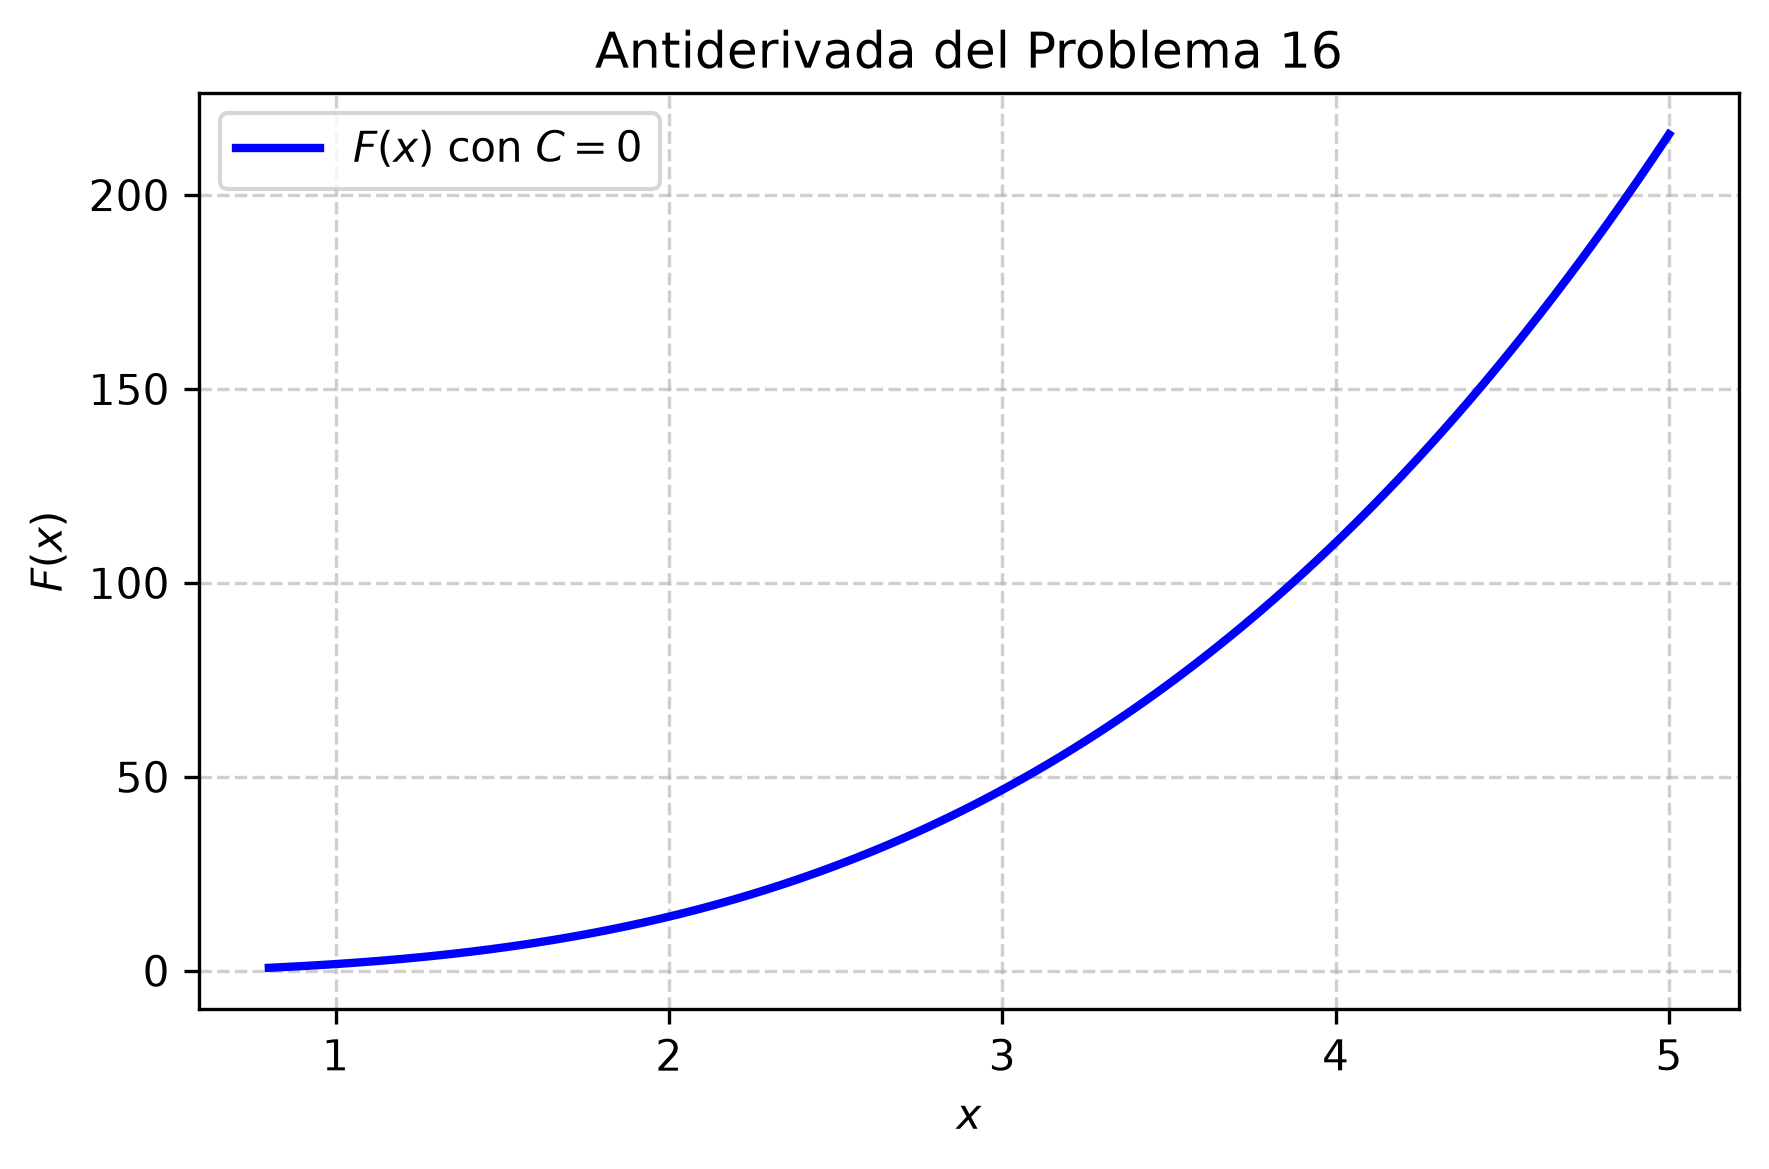
\includegraphics[width=\columnwidth]{semana_05/graficas/SEM05_P16_grafica.png}
	\caption{Representación gráfica de $f(x)$ y su antiderivada $F(x)$ evaluada para la constante de integración $C = 0$ (Problema 16).}
	\label{fig:problema16}
\end{figure}
